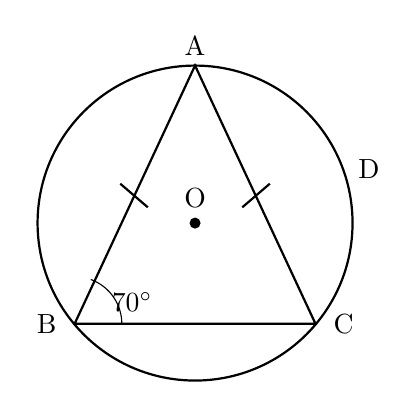
\begin{tikzpicture}[scale=1]

    % 1. Draw the circle centered at (0,0) with radius 2
    \draw[thick] (0,0) circle (2cm);

    % 2. Define coordinates
    \coordinate (O) at (0,0);        % Center of the circle
    \coordinate (A) at (0,2);        % Vertex A
    \coordinate (B) at (-1.53,-1.28); % Vertex B (on circle)
    \coordinate (C) at (1.53,-1.28);  % Vertex C (on circle)
    \coordinate (D) at (1.88,0.68);   % Point D on the arc AC

    % 3. Draw the triangle ABC
    \draw[thick] (A) -- (B) -- (C) -- cycle;

    % 4. Draw the dot for center O
    \fill (O) circle (2pt);

    % 5. Draw equal-length tick marks on AB and AC
    \draw[thick] (-0.95, 0.5) -- (-0.6, 0.2); % Tick on AB
    \draw[thick] (0.95, 0.5) -- (0.6, 0.2);   % Tick on AC

    % 6. Corrected 70 degree arc
    % We start from 0 degrees (the horizontal BC line) and sweep to 70 degrees
    \draw (B) ++(0:0.6) arc (0:70:0.6);
    % Position the label slightly outside the arc for clarity
    \node at (-0.8,-1.0) {$70^\circ$};

    % 7. Place labels for the points
    \node[above] at (A) {A};
    \node[left=3pt] at (B) {B};
    \node[right=3pt] at (C) {C};
    \node[right=2pt] at (D) {D};
    \node[above=2pt] at (O) {O};

\end{tikzpicture}